%----------------------------------------------------------------------------
\chapter*{4lang}\addcontentsline{toc}{chapter}{4lang}
%---
\section{The formalism}
The \texttt{4lang} system of semantic representation \cite{Kornai:2015a}
represents the meaning of linguistic units (both words and phrases)
as directed graphs of syntax-independent concepts.
Those representing binary relations are connected to their arguments
via edges labeled \texttt{1} and \texttt{2}, all other relations are treated
uniformly: \texttt{0}-edges represent attribution (\texttt{dog
	$\xrightarrow0$ large}), hypernymy (\texttt{dog $\xrightarrow0$ mammal}) and unary predication
(\texttt{dog  $\xrightarrow0$ bark}).
Concepts have no grammatical attributes and no event structure, e.g.
the phrases \textit{water freezes} and \textit{frozen water} would both be
represented as \textit{water}~$\xrightarrow0$~\textit{freeze}. 

The example in
Figure~\ref{fig:bird} shows the \texttt{4lang} definition of the
concept \texttt{bird}. This definition was built manually, as part of
the \texttt{4lang} dictionary \cite{Kornai:2013}, but similar
definitions have been created automatically from definitions of
monolingual dictionaries such as Longman, using the
\texttt{dict\_to\_4lang} tool \cite{Recski:2016d}.

The open-source 4lang pipeline\footnote{\url{https://github.com/kornai/4lang}}
contains tools for generating
directed graphs from raw text by mapping dependency edges in the output of the
Stanford parser \cite{deMarneffe:2006} to \texttt{4lang} subgraphs over
concepts corresponding to each word of the original sentence.
Optionally, the \texttt{4lang} system allows us to \textit{expand}
graphs, a process which unifies the graph with the definition graphs of
each concept. 
Besides being an open-source software library,
the \texttt{4lang} parser is also accessible via a public
REST API at \url{http://hlt.bme.hu/4lang}.

\begin{figure}
	\centering
	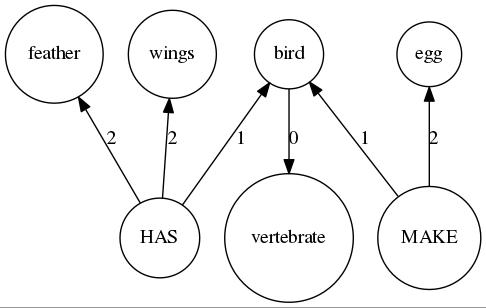
\includegraphics[scale=0.5]{figures/bird}
	\caption{4lang definition of \texttt{bird}.}
	\label{fig:bird}
\end{figure}

Graphs generated by the \texttt{4lang} parser have previously been used
successfully in measuring semantic similarity. The current state of the
art system on the \texttt{SimLex-999} benchmark \cite{Hill:2014a}
outperforms previous top systems by utilizing a simple similarity metric
between \texttt{4lang} definitions of pairs of English words
\cite{Recski:2016c}